\section{The \gls{fdtd}}
The aim of this section is to give the basic of numerical simulation by using \gls{fdtd} method, such that a speaker array sound propagation can be analysed. The method of using numerical simulate will be descried, such that the method can be adapted to one or more speaker in a sound pressure field. 
The theory behind \gls{fdtd} is to solve the wave equation by a finite-difference approximation for both time and space derivatives. This make it possible to easily simulate the sound pressure and particle velocity of a speaker at any time step. One advantage of using \gls{fdtd} is that the impulse response of a specified loudspeaker can be applied to the calculation, and therefore it is possible to simulate the speaker that is used in this project. For using \gls{fdtd} with a specified speaker, all simulation have to be done in a narrow frequency band, before the simulation give a good approximation, the \gls{fdtd} can not include the hole frequency band in one simulation. A second advantage of using \gls{fdtd} is that the calculation is preformed in time domain, which benefit from that the pressure and the particle velocity at a specified time step can be analyzed directly by solving two coupled equation.\citep{fdtddaga}\\


The two equation which need to be solved is the coupled first order equation of the pressure $p$ and the particle velocity $\vec{v}$. The first formula is the Euler \autoref{fdtd_euler}, which describe the relation between the gradient for the pressure $p$ and the derivative of the particle velocity $\vec{v}$ with respect to time \autoref{fdtd_euler}. 

\begin{equation}\label{fdtd_euler}
\frac{\partial \vec{v}}{\partial t} =- \frac{1}{\rho}\vec{\triangledown }p
\end{equation}

    \startexplain
    		\explain{$\rho$ is the density of the medium }{\si{\kilo\gram\per\cubic\meter}}
        \explain{$\partial t$ is an infinitesimal time step}{\si{\second}}
        \explain{$p$ is the pressure }{\si{\pascal}}
        \explain{$\vec{v}$ is the particle velocity}{\si{\meter\per\second}}
    \stopexplain

The \autoref{fdtd_euler} is only valid with small variation of pressure. The second \autoref{fdtd_linear} is the linear continuity equation. The equation describe the relation between derivative of pressure with respect of time and the velocity gradient. They are combined by the density of the medium and the speed of sound. 

 \begin{equation}\label{fdtd_linear}
\frac{\partial p}{\partial t} =- \rho c^2 \vec{\triangledown }\vec{v}
\end{equation}

    \startexplain
    		\explain{$\rho$ is the density of the medium }{\si{\kilo\gram\per\cubic\meter}}
        \explain{$\partial t$ is an infinitesimal time step}{\si{\second}}
        \explain{$p$ is the pressure }{\si{\pascal}}
        \explain{$c$ is the speed of sound }{\si{\meter\per\second}}
        \explain{$\vec{v}$ is the particle velocity}{\si{\meter\per\second}}
    \stopexplain

Both equation are approximated by using finite difference for every point in space and time, by using a 3 dimensional grid of the space. 


\subsection{\gls{fdtd} using Cartesian grid}

The Cartesian grid for \gls{fdtd} approximation is a well known technique, and will be used in this project \citep{finiteproblems}. The Cartesian grid is using the pressure \autoref{fdtd_linear} and the particle velocity \autoref{fdtd_linear} as the unknown quantities, which have to be solved for every point in space.  A small grid is visualized in \autoref{fig:fdtd_cartesian_grid}

\begin{figure}[H]
	\centering
\begin{picture}(0,0)%
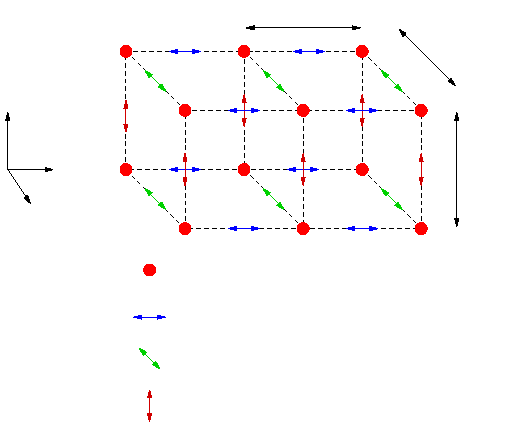
\includegraphics{fdtd_grid.pdf}%
\end{picture}%
\setlength{\unitlength}{4144sp}%
%
\begingroup\makeatletter\ifx\SetFigFont\undefined%
\gdef\SetFigFont#1#2#3#4#5{%
  \reset@font\fontsize{#1}{#2pt}%
  \fontfamily{#3}\fontseries{#4}\fontshape{#5}%
  \selectfont}%
\fi\endgroup%
\begin{picture}(3869,3327)(3541,-1288)
\put(6841,1649){$\delta y$}%
\put(3556,1244){$z$}%
\put(4006,704){$x$}%
\put(3826,344){$y$}%
\put(5806,1874){$\delta x$}%
\put(4996,-61){Pressure point}%
\put(4996,-421){Particle velocity x-direction}%
\put(4996,-781){Particle velocity y-direction}%
\put(4996,-1096){Particle velocity z-direction}%
\put(7066,704){$\delta z$}%
\end{picture}%
	\caption{A 3 dimensional example of Cartesian grid}
		\label{fig:fdtd_cartesian_grid}
\end{figure}


The grid points is build up on positions there is descried as $(i\,\delta x,j\,\delta y,k\,\delta z)$ at time $t=(l\pm\frac{1}{2})\delta t$, where the time step is visualized in \autoref{fig:fdtd_transient_point}

\begin{figure}[H]
	\centering
\begin{picture}(0,0)%
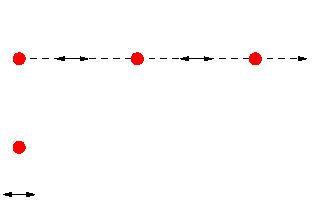
\includegraphics{fdtd_transient_point.pdf}%
\end{picture}%
\setlength{\unitlength}{4144sp}%
%
\begingroup\makeatletter\ifx\SetFigFont\undefined%
\gdef\SetFigFont#1#2#3#4#5{%
  \reset@font\fontsize{#1}{#2pt}%
  \fontfamily{#3}\fontseries{#4}\fontshape{#5}%
  \selectfont}%
\fi\endgroup%
\begin{picture}(2424,1594)(4898,-854)
\put(5176,469){$(l-\frac{1}{2})\delta t$}%
\put(5671, 29){$l\delta t$}%
\put(6516, 29){$(l+1)\delta t$}%
\put(6031,469){$(l+\frac{1}{2})\delta t$}%
\put(7246,254){$t$}%
\put(5266,-421){Pressure point}%
\put(5266,-781){Particle velocity}%
\end{picture}%
	\caption{Transient definition points of sound $p$ pressure and particle velocity $\vec{v}$}
		\label{fig:fdtd_transient_point}
\end{figure}

$\delta x,\delta y,\delta z$ is the spatial discretization step as shown in \autoref{fig:fdtd_cartesian_grid} and $\delta t$ is the time spatial discretization step as shown in \autoref{fig:fdtd_transient_point}. $i,j,k$ is the discrete indices for the point in grid and $l$ is the discrete time index. For every axis, the component of the particle velocity have to be determined at position in \autoref{fdtd_component} at time $t=(l\pm\frac{1}{2})\delta t$ \begin{equation}\label{fdtd_component}
\vec{v}= \begin{bmatrix}
v_x[(i\pm \frac{1}{2})\,\delta x,j\,\delta y,k\,\delta z]\\
v_y[i\,\delta x,(j\pm \frac{1}{2})\,\delta y,k\,\delta z]\\
v_z[i\,\delta x,j\,\delta y,(k\pm \frac{1}{2})\,\delta z]
\end{bmatrix}
\end{equation}
and the pressure is determined at position $p_{(i,j,k)}^{[l+1]}$. Since the used speaker in this project is a speaker used for air operation, the medium for $\rho$ in the calculation will be air \\


The following step is done to get the linearized equation for particle velocity in Cartesian grid to any time. First \autoref{fdtd_euler} has to be rewritten to \autoref{fdtd_euler_rewrite_system}.


\begin{subequations}\label{fdtd_euler_rewrite}
\begin{alignat}{2}
-\rho_0 \frac{\partial \vec{v}}{\partial t} &=\vec{\triangledown }p \label{fdtd_euler_rewrite_1}\\
-\rho_0 \frac{\partial \vec{v}}{\partial t} &=\frac{\partial p}{\partial x}\vec{x}+\frac{\partial p}{\partial y}\vec{y}+\frac{\partial p}{\partial z}\vec{z} \label{fdtd_euler_rewrite_2}
\end{alignat}
\end{subequations}
Since $\vec{v}$ is a equation system of three inputs, the \autoref{fdtd_euler_rewrite} is splittet to a equation system \citep{Sakuma2014}.

\begin{subequations}\label{fdtd_euler_rewrite_system}
\begin{alignat}{2}
\frac{\partial p}{\partial x} &=-\rho_0 \frac{\partial v_x}{\partial t} \label{fdtd_euler_rewrite_system_1}\\
\frac{\partial p}{\partial y} &=-\rho_0 \frac{\partial v_y}{\partial t} \label{fdtd_euler_rewrite_system_2}\\
\frac{\partial p}{\partial z} &=-\rho_0 \frac{\partial v_z}{\partial t} \label{fdtd_euler_rewrite_system_2}
\end{alignat}
\end{subequations}


Next the $v_x$, $v_y$ and $v_z$ have to be differentiated with respect to $t$ and $p$ with respect to $x$, $y$ and $z$. To make it simple when differentiate with $t$ \autoref{fdtd_euler_diff_1} for all $v_x$, $v_y$ and $v_z$ only the $v_x$ is showed. The differentiation with $v_y$ and $v_z$ is similar but only the indices is at there respectively indices. When differentiate with respect to $x$, $y$ and $z$ in \autoref{fdtd_linear_diff_2} only the differentiate with respect to $x$ is done. The differentiation with respect to $y$ and $z$ is similar but only the indices is at there respectively indices \citep{Sakuma2014}.



\begin{subequations}\label{fdtd_euler_diff}
\begin{alignat}{2}
\frac{\partial v_x}{\partial t}\mid _{(i+\frac{1}{2},j,k)}^{[l]} &= \frac{(v_x)_{(i+\frac{1}{2},j,k)}^{[l+\frac{1}{2}]} -(v_x)_{(i+\frac{1}{2},j,k)}^{[l-\frac{1}{2}]}}{\delta t} \label{fdtd_euler_diff_1} \\
\frac{\partial p}{\partial x}\mid _{(i+\frac{1}{2},j,k)}^{[l]} &= \frac{p_{(i+1,j,k)}^{[l]} -p_{(i,j,k)}^{[l]}}{\delta x}  \label{fdtd_linear_diff_2}
\end{alignat}
\end{subequations}

Substituting \autoref{fdtd_euler_diff} intro \autoref{fdtd_euler_rewrite_system} and solve for $(v_x)_{(i+\frac{1}{2},j,k)}^{[l+\frac{1}{2}]}$ leads to following three \autoref{fdtd_particle_velocity}


\begin{subequations}\label{fdtd_particle_velocity}
\begin{alignat}{2}
(v_x)_{(i+\frac{1}{2},j,k)}^{[l+\frac{1}{2}]}&= (v_x)_{(i+\frac{1}{2},j,k)}^{[l-\frac{1}{2}]}-\frac{\delta t}{\rho_0 \delta x} \left( p_{(i+1,j,k)}^{[l]} -p_{(i,j,k)}^{[l]}  \right)\\
(v_y)_{(i,j+\frac{1}{2},k)}^{[l+\frac{1}{2}]}&= (v_y)_{(i,j+\frac{1}{2},k)}^{[l-\frac{1}{2}]}-\frac{\delta t}{\rho_0 \delta y} \left( p_{(i,j+1,k)}^{[l]} -p_{(i,j,k)}^{[l]}  \right)\\
(v_z)_{(i,j,k+\frac{1}{2})}^{[l+\frac{1}{2}]}&= (v_z)_{(i,j,k+\frac{1}{2})}^{[l-\frac{1}{2}]}-\frac{\delta t}{\rho_0 \delta z} \left( p_{(i,j,k+1)}^{[l]} -p_{(i,j,k)}^{[l]}  \right)
\end{alignat}
\end{subequations}
\\

The following step is done to get the linearized equation for pressure in Cartesian grid to any time. First \autoref{fdtd_linear} has to be rewritten to \autoref{fdtd_linear_rewrite_2}

\begin{subequations}\label{fdtd_linear_rewrite}
\begin{alignat}{2}
- \frac{1}{\rho_0c^2} \frac{\partial p}{\partial t} &=\vec{\triangledown }\vec{v} \label{fdtd_linear_rewrite_1}\\
- \frac{1}{\rho_0c^2} \frac{\partial p}{\partial t} &=\frac{\partial v_x}{\partial x}+\frac{\partial v_y}{\partial y}+\frac{\partial v_z}{\partial z}\label{fdtd_linear_rewrite_2}
\end{alignat}
\end{subequations}
\\


Next the $p$ have to be differentiated with respect to $t$ and $v_x$, $v_y$ and $v_z$ with respect to $x$, $y$ and $z$ respectively as done in \autoref{fdtd_linear_diff}. As in \autoref{fdtd_euler_diff} only the differentiation to $t$ and $x$ is done \citep{Sakuma2014}.



\begin{subequations}\label{fdtd_linear_diff}
\begin{alignat}{2}
\frac{\partial p}{\partial t}\mid _{(i,j,k)}^{[l+\frac{1}{2}]} &= \frac{p_{(i,j,k)}^{[l+1]} -p_{(i,j,k)}^{[l]}}{\delta t} \label{fdtd_linear_diff_1}\\
\frac{\partial v_x}{\partial x}\mid _{(i,j,k)}^{[l+\frac{1}{2}]} &= \frac{(v_x)_{(i+\frac{1}{2},j,k)}^{[l+\frac{1}{2}]} -(v_x)_{(i-\frac{1}{2},j,k)}^{[l+\frac{1}{2}]}}{\delta x} \label{fdtd_euler_diff_2}
\end{alignat}
\end{subequations}


Substituting \autoref{fdtd_linear_diff} intro \autoref{fdtd_linear_rewrite_2} and solve for $p_{(i,j,k)}^{[l+1]}$ leads to  \autoref{fdtd_pressure}




\begin{multline}\label{fdtd_pressure}
p_{(i,j,k)}^{[l+1]} = p_{(i,j,k)}^{[l]} - \rho_0 c^2 \delta t \Biggl( \frac{(v_x)_{(i+\frac{1}{2},j,k)}^{[l+\frac{1}{2}]} - (v_x)_{(i-\frac{1}{2},j,k)}^{[l+\frac{1}{2}]}}{\delta x} \\ 
+ \frac{(v_y)_{(i,j+\frac{1}{2},k)}^{[l+\frac{1}{2}]}-(v_y)_{(i,j-\frac{1}{2},k)}^{[l+\frac{1}{2}]}}{\delta y} +  \frac{(v_z)_{(i,j,k+\frac{1}{2})}^{[l+\frac{1}{2}]}-(v_z)_{(i,j,k-\frac{1}{2})}^{[l+\frac{1}{2}]}}{\delta z} \Biggr)
\end{multline}




\subsection{\gls{fdtd} stability conditions}




